\chapter{Componente Processor Expert}

\label{sec:ProcessorExpert}

\section{Porturi de intrare și ieșire}

\begin{wrapfigure}{l}{0.5\textwidth}
    \vspace{-30pt}
    \center{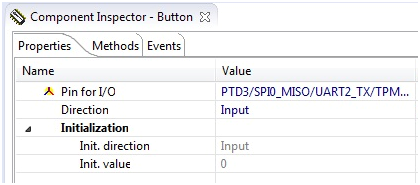
\includegraphics[width=0.5 \textwidth]{images/BitIO.png}}
    \vspace{-15pt}
    \caption{\label{fig:CodeWarrior-BitIO} Configurarea unui port de intrare / ieșire}
    \vspace{-10pt}
\end{wrapfigure}

Cu ajutorul componentei \textit{BitIO} din Processor Expert putem accesa porturi de intrare și iesire ale microcontroller-ului, folosind pinii configurabili ai acestuia. O astfel de componentă este caracterizată de un nume, de un pin al microcontrollerului pe care este mapată, o direcție (portul poate fi de intrare sau de ieșire) și valoarea inițiala, în cazul pinilor configurați pentru ieșire. Cu o astfel de componentă se poate controla foarte ușor un LED, spre exemplu.

\subsection{Porturi de ieșire}

\begin{wrapfigure}{r}{0.5\textwidth}
    \vspace{-60pt}
    \center{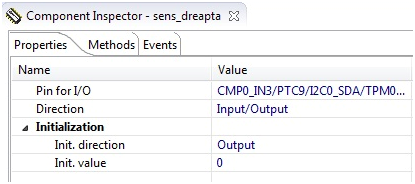
\includegraphics[width=0.5 \textwidth]{images/PExOutputIO.png}}
    \vspace{-20pt}
    \caption{\label{fig:CodeWarrior-PExOutputIO} Utilizarea unei componente}
    \vspace{-10pt}
\end{wrapfigure}

În figura \ref{fig:CodeWarrior-PExOutputIO} se poate regăsi un exemplu de utilizare al acestei componente. După cum vă puteți da seama, \textit{Init. direction} vine să specifice tipul portului, iar \textit{Init. value} valoarea inițială a acestuia.

Următoarele metode sunt puse la dispoziție pentru un programator în vederea controlării unui astfel de port:
\begin{description}
    \item[void SetVal(void), void ClrVal(void)] Acestea permit setarea portului de ieșire la valoarea \textit{"high"}, respectiv \textit{"low"}. 
    \item[void NegVal(void)] Metoda permite negarea unei valori setate ca output. Din 0 se poate se poate trece în 1 și invers. Cu ajutorul acestei metode se poate face un led, de exemplu, să blinkăie.
    \item[void PutVal(bool Val)] Metoda permite setarea valorii de ieșire pe un pin de ieșire.
    \item[void SetDir(bool Dir)] Setează direcția unui pin. Dacă parametrul are valoarea FALSE, pin-ul este marcat ca fiind pin de intrare (un buton, spre exemplu), iar dacă are valoarea TRUE, atunci el devine pin de ieșire.
\end{description}

De asemenea, mai jos avem și un exemplu simplu de utilizare al acestei componente:

\lstinputlisting[caption=Exemplu de utilizare a unui BitIO, style=customc]{sources/exampleBitIO.lst}

\subsection{Porturi de intrare}

Următoarele metode sunt puse la dispoziție pentru un programator în vederea controlării unui astfel de port:

\begin{description}
    \item[bool GetVal(void)] Întoarce valoarea pinului de intrare: FALSE pentru "0", respectiv TRUE pentru "1". În cazul unui buton, obținerea valorii "0" înseamnă că butonul este apăsat.
\end{description}

Citirea valorii unui port de intrare, se poate face într-o buclă infinită, așa cum arată exemplul următor:

\lstinputlisting[caption=Citirea stării unui buton în buclă, style=customc]{sources/exampleBitIORead.lst}

\newpage

\subsection{Componenta de așteptare (Wait)}

\begin{wrapfigure}{l}{0.5\textwidth}
    \vspace{-25pt}
    \center{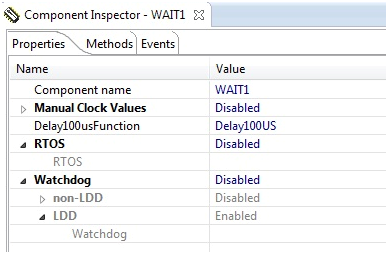
\includegraphics[width=0.5 \textwidth]{images/Wait.png}}
    \vspace{-20pt}
    \caption{\label{fig:CodeWarrior-Wait} Configurarea componentei Wait}
    \vspace{-10pt}
\end{wrapfigure}

Processor Expert pune la dispoziție o componentă ce implementează o rutină wait, prin intermediul căreia putem introduce o întârziere în cadrul execuției programului nostru. De exemplu, dacă vrem ca led-ul nostru să se aprindă și să se stingă la fiecare 5 secunde vom apela rutinele definite mai sus, secvențial, folosind ca și pas intermediar această componentă. În timp ce ne aflăm în această rutină de așteptare, doar întreruperile mai pot produce ieșirea din rutină.

Mai jos sunt definite și explicate câteva dintre proprietățile acestei componente:

\begin{description}
    \item[Component Name] reprezintă numele sub care componenta se regăsește în codul sursă. Deoarece este foarte posibil ca, în cadrul aplicației noastre, să avem mai multe componente de același tip, numele va fi folosit ca diferențiator. În plus, ar mai trebui să știți că toate metodele unei componente sunt prefixate, în mod implicit, cu numele componentei de care aparțin.
    \item[Manual clock values] permite obținerea tactului de ceas fie de la CPU (opțiunea implicită, așa o vom folosi noi), fie de la o valoare specificată manual.
    \item[Delay100usFunction] menționează funcția ce furnizează o întârziere de 100 microsecunde. Se va folosi funcția specificată în imaginea de mai sus.
    \item[RTOS] este parametrul prin care componenta este informată dacă un sistem de operare este folosit în sistem (sistem de operare în timp real). În cazul nostru, ar reprezenta un overhead utilizarea unui sistem de operare, având în vedere că acesta ar fi util doar dacă avem o aplicație ce necesită support de multitasking.
\end{description}

Cum sistemul nostru nu folosește watchdogs, parametrul \textbf{WatchDog} trebuie configurat pe modul dezactivat.

Componenta poate fi folosită prin accesarea metodelor prezentate succint mai jos:

\begin{description}
    \item[void WaitCycles(word cycles)] parametrul specifică câți cicli de procesor se așteaptă;
    \item[void Waitms(word ms)] parametrul specifică câte milisecunde se va așteapta până la executarea următoarei instrucțiuni din programul nostru;
    \item[void Waitus(word us)] parametrul specifică câte microsecunde se așteaptă;
\end{description}

\textcolor{red}{Notă:} Există două clase de metode pentru componenta Wait. Unele permit specificarea numărului de secunde cât se așteaptă, celelalte operează cu cicli de ceas.

\subsection{Componenta Timer}

Folosind o componentă de tip \textit{Timer}, pusa la dispoziție de \textit{Processor Expert}, putem măsura ușor trecerea timpului. Timerul, după cum îi spune și numele, oferă facilitatea de a măsura intervale fixe de timp și de a genera întreruperi la expirarea intervalului măsurat. Un timer, odată inițializat va funcționa independent de unitatea centrală (core-ul microprocesorului). Acest lucru permite eliminarea buclelor de întârziere din programul principal.

Principiul de funcționare a unui \textit{Timer} poate fi descris în linii mari de cele trei unități:

\begin{enumerate}
    \item \textbf{Registrul numărător (Timer Counter)} - măsoară efectiv intervalele de timp și este incrementat automat cu o frecvență cunoscută.
    \item \textbf{Prescaler-ul} - are rolul de a diviza în funcție de necesitățile aplicației frecvența de ceas. În acest fel, registrul numărător poate fi incrementat mai repede sau mai încet.
    \item La fiecare incrementare a TCNT are loc o comparație între acest registru și o valoare stocată într-un alt registru - numit registru comparator. Valoarea din registrul comparator poate fi încărcată de către programator prin scrierea lui. Dacă are loc egalitatea se generează o întrerupere, în caz contrar incrementarea continuă.
\end{enumerate}

\begin{wrapfigure}{r}{0.5\textwidth}
    \vspace{-30pt}
    \center{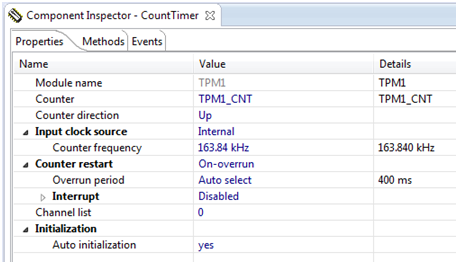
\includegraphics[width=0.5 \textwidth]{images/Timer.png}}
    \vspace{-20pt}
    \caption{\label{fig:CodeWarrior-Timer} Configurarea unui timer}
    \vspace{-10pt}
\end{wrapfigure}

Timerele sunt prevăzute cu mai multe canale astfel încât se pot desfășura diferite număratori în paralel. Vă invităm să vă documentați asupra numărului de timere și de canale pe care placa de dezvoltare FRDM-KL25Z le pune la dispoziție, pentru că aceasta este placa pe care veți dezvolta aplicația. De asemenea, timerele pot funcționa și în moduri PWM, astfel încât să genereze pe un pin de ieșire un semnal. Mai multe detalii veți afla în paragrafele următoare.

Proprietăți ale componentei:

\begin{description}
    \item[Component Name] reprezintă numele sub care componenta se regăsește în codul sursă.
    \item[Counter Direction] permite specificarea direcției în care se numără: registrul numărător se incrementează sau se va decrementa?
    \item[Counter Frequency] definește granularitatea cu care se numără. Numărătorul incrementeaza valoarea counter-ului în funcție de această frecvență. De exemplu, dacă setăm frecvența la 1 kHz, într-o secundă, numărătorul ajunge la valoarea 1000. 
\end{description}

Metode de interfațare:

\begin{description}
    \item[$LLD\_Error$ ResetCounter(LDD\_TDeviceData *DeviceDataPtr)] inițializează la 0 (resetează) counter-ul. În cazul proiectului nostru, parametrul \textit{DeviceDataPtr} poate fi setat la \textit{NULL}. Funcția întoarce ERR\_OK dacă totul a decurs bine și ERR\_SPEED în caz de eroare. 
    \item[TValueType GetCounterValue(LDD\_TDeviceData *DeviceDataPtr)] această funcție returnează valoarea registrului contor (numărul de pulsuri de ceas înregistrate de la ultima operație de \textit{Reset}). În cazul proiectului nostru, parametrul \textit{DeviceDataPtr} poate fi setat pe NULL.
\end{description}

Iată și un exemplu simplu de utilizare:

\lstinputlisting[caption=Utilizarea unui Timer, style=customc]{sources/exampleTimer.lst}

\subsection{Componenta PWM (Pulse Width Modulation)}

\textit{PWM (Pulse Width Modulation)} este o tehnică folosită pentru a varia în mod controlat tensiunea dată unui dispozitiv electronic. Această metodă schimbă foarte rapid tensiunea oferită dispozitivului respectiv din \textit{ON} în \textit{OFF} și invers. Perioada de timp corespunzătoare valorii ON dintr-un ciclu ON-OFF se numește factor de umplere (în engleză - \textit{duty cycle}) și reprezintă, in medie, ce tensiune va primi dispozitivul electronic. Astfel, se pot controla circuitele analogice din domeniul digital. Practic, asta înseamnă că un LED acționat astfel se va putea aprinde / stinge gradual, iar în cazul unui motor acesta se va roti mai repede sau mai încet.

Factorul de umplere se exprimă în procente și reprezintă cât la sută din perioada unui semnal acesta va fi pe nivelul ON. Modularea folosește variația factorului de umplere a unei forme de undă dreptunghiulară pentru a genera la ieșire o tensiune analogică. Așadar, putem control o variabilă prin intermediul alteia. De exemplu, putem controla amplitudinea unei sinusoide (numită purtătoare) cu un alt semnal (rezultând modulatie în amplitudine - AM). A nu se confunda cu combinarea (mixarea) a două semnale, unde semnalele sunt pur și simplu adunate.

\begin{figure}
    \centering
    \subfloat[]{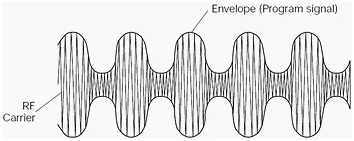
\includegraphics[width=3.1in]{images/Modulation1.png}} 
    \subfloat[]{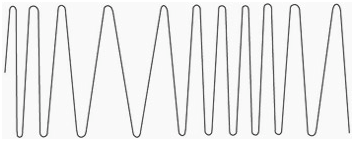
\includegraphics[width=3.1in]{images/Modulation2.png}}
    \caption{Modulație în amplitudine (a) și în frecvență (b)} 
    \label{fig:CodeWarrior-Modulation} 
\end{figure} 

\subsubsection{Modificarea turației unui motor}

\begin{wrapfigure}{r}{0.3\textwidth}
    \vspace{-20pt}
    \center{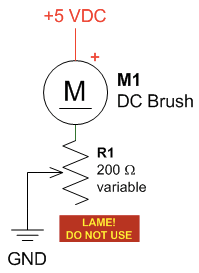
\includegraphics[width=0.3 \textwidth]{images/ResistenceMethod.png}}
    \vspace{-15pt}
    \caption{\label{fig:CodeWarrior-ResistenceMethod} Controlarea unui motor folosind o rezistență}
    \vspace{-10pt}
\end{wrapfigure}

Să presupunem că avem un motor ce funcționează la o anumită tensiune, în curent continuu. Aplicându-i acea tensiune, motorul va funcționa la o anumită turație. Ce facem dacă vrem să-i modificăm turația? O variantă este să folosim roți dințate, dar dacă am vrea să-l controlam prin metode electrice? Cea mai simpla (și ineficientă) formă de a controla turația unui motor în curent continuu este folosirea unei rezistențe. Este ineficientă deoarece multă energie este pierdută, transformându-se în căldură.

Dacă înlocuim rezistența cu un tranzistor, putem controla turația (viteza) motorului aplicând în baza tranzistorului un semnal - cât timp semnalul este "high", tranzistorul închide circuitul motorului către masă. Când semnalul din baza tranzistorului este pe "low", prin motor nu trece curent. Pierderi de putere apar acum (față de exemplul anterior, în care foloseam o rezistență) doar la trecerea între semnalul "high" și cel "coborât" - iar timpul petrecut în aceste faze tranzitorii este foarte scurt.

\begin{wrapfigure}{r}{0.3\textwidth}
    \vspace{-60pt}
    \center{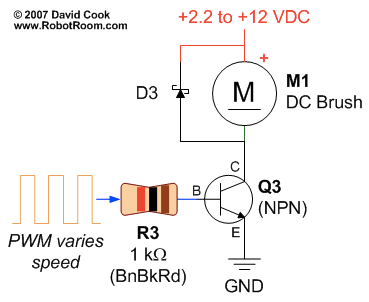
\includegraphics[width=0.3 \textwidth]{images/TransistorMethod.png}}
     \vspace{-15pt}
    \caption{\label{fig:CodeWarrior-TransistorMethod} Controlarea unui motor folosind un tranzistor}
    \vspace{-10pt}
\end{wrapfigure}

Motorul are o anumită inerție, astfel încât nu pornește sau se oprește brusc. De aceea, controlarea tranzistorului printr-un semnal drepunghiular cu o frecvență suficient de mare (semnificativ mai mare decât timpul de răspuns al motorului) nu produce "smucituri" în funcționarea motorului. În același mod putem controla intensitatea luminii generate de un led. Ca și o curiozitate, dacă folosim în baza tranzistorului o frecvență în spectrul auzului uman, vom sfârși prin a auzi un bazâit. De aceea, dacă este posibil, e bine ca frecvența folosită să fie peste 20 kHz. Și nu uitați de câini, care aud la frecvențe și mai mari de 20 kHz!

\subsubsection{Generarea unui semnal PWM în mediu digital}

Majoritatea microcontrollerelor pot genera semnale PWM (pe un pin de ieșire) folosind un numărător ce este incrementat automat cu o anumita cadență până ajunge la o anumită valoare - când este resetat și procesul se reia. Într-o astfel de perioadă, semnalul pe pinul de ieșire este "low" (sau "high") până când numărătorul ajunge la o valoare și apoi este comutat în cealaltă stare. În acest fel creăm un semnal dreptunghiular, cu care vom controla motorul.

\begin{wrapfigure}{r}{0.5\textwidth}
    \vspace{-20pt}
    \center{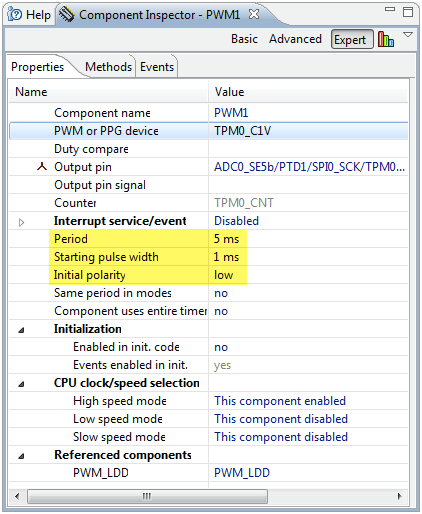
\includegraphics[width=0.5 \textwidth]{images/PExPWM.png}}
    \vspace{-15pt}
    \caption{\label{fig:CodeWarrior-PExPWM} Configurarea unei componente de tip PWM}
    \vspace{-30pt}
\end{wrapfigure}

\subsubsection{Processor Expert și generarea de semnal PWM}

Proprietăți ale componentei:

\begin{description}
    \item[Component Name] element de identificare al componentei;
    \item[Output Pin] este pinul fizic pe care este mapată componentă;
    \item[Period] în mod evident, reprezintă perioada semnalului PWM;
    \item[Starting Pulse Width] este timpul setat pentru prima parte din duty cycle; 
    \item[Initial Polarity] definește dacă prima parte a duty cycle-ului este ON sau OFF;
    \item[Initialization] specifică dacă la inițializare / resetare componenta este sau nu activată. Dacă nu este activată, ieșirea pe pin este setată la valoarea definită prin \textit{"Initial Polarity"}. În acest caz, pentru a o activa programatic, trebuie folosită metoda \textit{Enable}; 
\end{description}

\textcolor{red}{Notă:} Pentru modificarea programatică a duty cycle-ului, Processor Expert pune la dispoziție mai multe metode, noi folosind \textbf{void SetRatio16(word ratio)}.

Metode de interfațare:

\begin{description}
    \item[byte Enable / Disable (void)] metodele pornesc / opresc componenta (generarea de semnal). Valoarea întoarsă poate fi ERR\_OK sau ERR\_SPEED.
    \item[byte SetRatio16(word ratio)] aceasta metodă setează un nou duty cycle pentru componentă. Ratio este o valoare unsigned, cuprinsă între 0x0 și 0xffff (65535), proporțională cu procentul 0 - 100\%. Valoarea întoarsă poate fi ERR\_OK sau ERR\_SPEED.
    \item[byte SetValue(void), byte ClrValue(void)] permit setarea directă a pinului de ieșire atunci când componenta este oprită (folosind metoda \textit{Disable}, în prealabil). Valoarea întoarsă poate fi ERR\_OK, ERR\_SPEED sau ERR\_ENABLE.
\end{description}

O dată instanțiată o componentă de acest tip, funcțiile oferite pot fi folosite așa cum sunt utilizate mai jos:

\lstinputlisting[caption=Utilizarea funcțiilor puse la dispozție de componenta PWM, style=customc]{sources/examplePWM.lst}

\subsubsection{Controlul sensului de rotație al motorului}

Cu ajutorul unui semnal PWM putem modula viteza de rotație a unui motor. Este important, de asemenea, să controlăm și sensul în care motorul se rotește. Acest lucru îl vom realiza prin intermediul unui pin de ieșire al microprocesorului conectat la fiecare punte H ce comanda un motor. În funcție de valoarea acestui pin (0 sau 1) stabilim direcția în care se învârte motorul.

\subsubsection{Logică inversată}

Placa de dezvoltare FRDM-KL25Z și motoarele folosite în cadrul acestui proiect funcționează după o logică inversată. Îți aduci aminte ce înseamna "duty cycle"? Dacă nu, îți mai aducem noi aminte încă o dată, însemna că viteza motorului era mai mare cu cât semnalul nostru stătea mai mult timp în "high" (1 logic) într-o perioada. Ehh, gândeste-te acum exact invers – în loc să conteze cât stă în "high", contează cât stă în "low" (0 logic).

